\chapter{Analiza i projektowanie systemu}
\label{cha:projektowanie}

\section{Wymagania systemowe}
\label{sec:wymagania}
Proces projektowania asystenta AI wymagał w pierwszej kolejności zdefiniowania jednoznacznych wymagań, które system musi spełniać, aby sprostać zidentyfikowanym problemom biznesowym i technicznym. Zebrano je i podzielono na wymagania funkcjonalne (określające, co system ma robić) oraz niefunkcjonalne (określające, jak system ma działać pod kątem jakości, wydajności i ograniczeń technicznych).

\subsection{Wymagania funkcjonalne}
\label{subsec:wymagania_funkcjonalne}
Do najważniejszych wymagań funkcjonalnych stawianych przed systemem należą:
\begin{itemize}
	\item \textbf{Zarządzanie grupami urządzeń:} Użytkownik musi mieć możliwość utworzenia nowej grupy w systemie (otrzymując unikalny kod dostępu) oraz dołączenia do istniejącej grupy z poziomu dowolnego urządzenia klienckiego.
	\item \textbf{Zarządzanie wtyczkami (ang. \textit{plugins}):} Aplikacja kliencka musi automatycznie wykrywać i ładować skompilowane wtyczki (pliki \texttt{.dll}) z określonego katalogu lokalnego. Użytkownik może z poziomu interfejsu klienta instalować, włączać oraz wyłączać poszczególne wtyczki.
	\item \textbf{Przetwarzanie zapytań w języku naturalnym:} System musi umożliwić użytkownikowi wprowadzanie poleceń tekstowych lub głosowych z poziomu dowolnego urządzenia należącego do grupy.
	\item \textbf{Agregacja możliwości urządzeń:} Serwer centralny musi posiadać funkcję agregowania metadanych wszystkich aktywnych wtyczek i ich funkcji dla całej grupy urządzeń, w celu przekazania ich jako kontekstu do modelu LLM.
	\item \textbf{Autoryzacja wykonania funkcji:} Przed rozesłaniem poleceń wykonawczych (RPC) do klientów, serwer powinien zaprezentować użytkownikowi listę zinterpretowanych intencji (funkcji do wywołania wraz z argumentami) w celu ich weryfikacji i zatwierdzenia.
	\item \textbf{Rozproszone wykonanie zadania:} Po akceptacji przez użytkownika, system musi przekazać żądania wywołania funkcji do odpowiednich urządzeń, zebrać wyniki i zaprezentować je użytkownikowi.
\end{itemize}

\subsection{Wymagania niefunkcjonalne}
\label{subsec:wymagania_niefunkcjonalne}
Z perspektywy architektury oraz środowiska wykonawczego, zdefiniowano następujące wymagania niefunkcjonalne:
\begin{itemize}
	\item \textbf{Rozszerzalność (ang. \textit{Extensibility}):} System musi pozwalać na wdrażanie nowych funkcjonalności (obsługi nowych urządzeń lub akcji) bez konieczności rekonfiguracji, zatrzymywania lub modyfikacji kodu źródłowego serwera.
	\item \textbf{Komunikacja o niskich opóźnieniach:} Opóźnienia w dystrybucji poleceń z serwera do urządzeń klienckich nie mogą przekraczać wartości akceptowalnych dla interaktywnych systemów sterowania. Wymusza to użycie technologii działającej w czasie rzeczywistym, takiej jak WebSocket.
	\item \textbf{Agnostyczność wobec dostawców AI:} Mechanizm mapowania zapytań języka naturalnego na struktury danych musi być niezależny od konkretnego dostawcy modelu sztucznej inteligencji, pozwalając na łatwą zmianę silnika LLM.
	\item \textbf{Modularność logiki po stronie serwera:} Kod serwera musi być ustrukturyzowany w sposób umożliwiający łatwy podział i odseparowanie poszczególnych domen wiedzy (zgodnie z architekturą modułową).
\end{itemize}

\section{Modelowanie przypadków użycia systemu}
\label{sec:przypadki_uzycia}

\subsection{Identyfikacja aktorów i głównych procesów biznesowych}
\label{subsec:aktorzy}
Podczas modelowania przypadków użycia (ang. \textit{Use Cases}) zidentyfikowano głównego aktora systemu: \textbf{Użytkownika końcowego}. Wchodzi on w interakcję z systemem za pośrednictwem aplikacji klienckiej (np. komputera, telefonu). Do aktorów systemowych (pomocniczych) należą również \textbf{Zewnętrzny model LLM}, z którym komunikuje się serwer centralny w celu parsowania intencji.

Główny proces biznesowy to „Zlecenie wykonania rozproszonego zadania”, w którym użytkownik wypowiada komendę (np. „Wycisz mój telefon i uruchom przeglądarkę na komputerze”). System, na podstawie połączonych metadanych urządzeń w grupie, interpretuje to jako dwa niezależne wywołania funkcji, żąda potwierdzenia od użytkownika i koordynuje równoległe ich wykonanie.

\subsection{Diagramy przypadków użycia}
\label{subsec:diagramy_uc}
W celu wizualizacji kluczowych interakcji użytkownika z aplikacją kliencką oraz serwerem, opracowano diagram przypadków użycia w standardzie UML. Przypadki te obejmują między innymi tworzenie grupy, synchronizację stanu połączenia, zarządzanie lokalnymi wtyczkami oraz cykl życia samego promptu.

\begin{figure}[H]
	\centering
	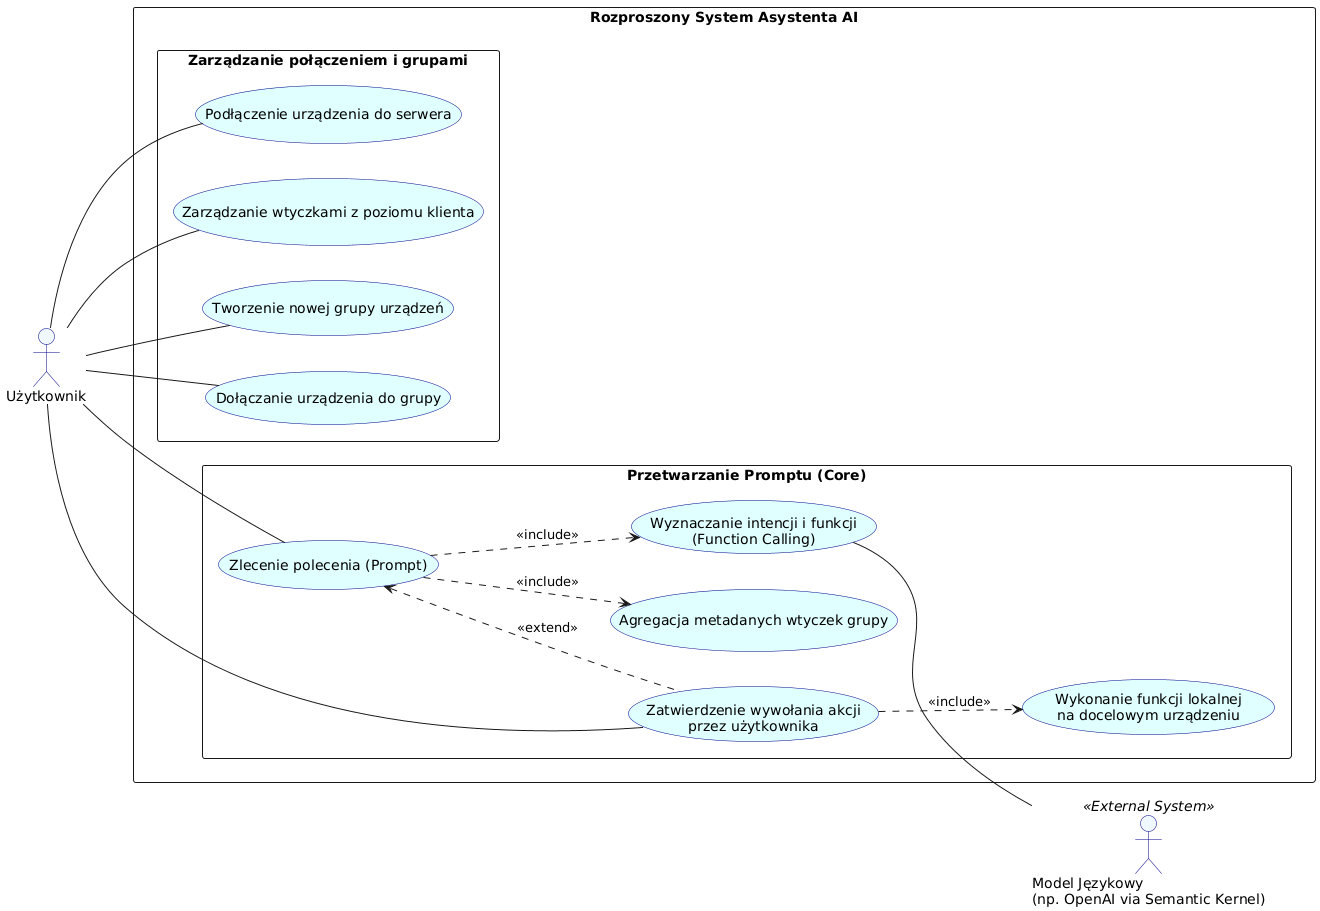
\includegraphics[width=0.8\textwidth]{figures/use-case-diagram.png}
	\vspace{5cm}
	\caption{Diagram przypadków użycia dla systemu asystenta AI}
	\label{fig:use_case}
\end{figure}

\section{Architektura systemu}
\label{sec:architektura}
Zgodnie z założeniami zdefiniowanymi w analizie teoretycznej (zob. Rozdział \ref{cha:analiza_dziedziny}), system operuje w oparciu o architekturę klient-serwer. Logika biznesowa została wyraźnie rozdzielona pomiędzy centralny punkt koordynacyjny a agentów wykonawczych wyposażonych w dynamiczne moduły.

\subsection{Architektura Modular Monolith i podział na konteksty (ang. \textit{Bounded Contexts})}
\label{subsec:modular_monolith}
Aplikacja serwerowa implementuje wzorzec modułowego monolitu. Główny proces został logicznie podzielony na hermetyczne obszary (ang. \textit{Bounded Contexts}), co gwarantuje wysoką spójność wewnętrzną. Wyróżniono następujące moduły:
\begin{itemize}
	\item \textbf{Connection:} Zarządza tożsamością urządzeń i żywotnością fizycznych połączeń opartych na protokole WebSockets.
	\item \textbf{Groups:} Implementuje logikę biznesową powiązaną z tworzeniem przestrzeni współdzielonych i generowaniem kodów dostępu.
	\item \textbf{Plugins:} Agreguje nadsyłane z klientów struktury danych opisujące interfejsy wtyczek.
	\item \textbf{Prompts:} Odpowiada za bezpośrednią integrację z warstwą sztucznej inteligencji, budując kontekst i mapując wyniki przy użyciu warstwy pośredniczącej.
	\item \textbf{Tasks:} Śledzi przepływ zdalnych wywołań od momentu zlecenia aż do odebrania wyniku (lub błędu) z urządzenia końcowego.
\end{itemize}

\subsection{Struktura warstwowa modułów (DDD i CQRS)}
\label{subsec:ddd_cqrs}
Wewnętrzna struktura każdego z wymienionych modułów opiera się na czterech warstwach: aplikacyjnej (\textit{Application}), domenowej (\textit{Domain}), infrastruktury (\textit{Infrastructure}) oraz integracyjnej (\textit{Integration}). Modele i reguły biznesowe izolowane są w warstwie domeny, która pozbawiona jest zewnętrznych zależności technicznych. Dostęp do operacji aplikacyjnych realizowany jest z wykorzystaniem wzorca CQRS (ang. \textit{Command Query Responsibility Segregation}), oddzielając komendy mutujące stan (np. \textit{CreateGroupCommand}) od zapytań (np. \textit{GetGroupDetailsQuery}). Wymiana informacji między modułami, aby zachować ich niezależność, przebiega w pełni asynchronicznie poprzez publikację zdarzeń (ang. \textit{Integration Events}).

\subsection{Architektura wtyczek na urządzeniach klienckich}
\label{subsec:architektura_wtyczek}
Aplikacja kliencka pełni rolę środowiska wykonawczego. Główny proces programu przy starcie skanuje zawartość katalogu \texttt{plugins/}. Po wykryciu skompilowanej biblioteki \texttt{.dll}, aplikacja za pomocą mechanizmu \textit{Reflection} ładuje moduł i ekstrahuje metadane (nazwy i opisy klas, metod oraz ich parametrów wejściowych). Serwer nigdy nie dysponuje binarnym kodem wtyczki, zapewniając tym samym wysoki stopień separacji bezpieczeństwa i elastyczność dystrybucji oprogramowania po stronie użytkownika.

\section{Projekt bazy danych}
\label{sec:baza_danych}

\subsection{Modelowanie danych z perspektywy domenowej}
\label{subsec:modelowanie_domenowe}
Zgodnie z zasadami DDD, model bazy danych oparty jest na persystencji zamkniętych agregatów. Oznacza to, że baza danych operuje raczej na spójnych stanach całych obiektów biznesowych (np. \textit{Grupa} zawierająca powiązane informacje autoryzacyjne) niż na zdenormalizowanych tabelach silnie złączonych kluczami obcymi ponad granicami poszczególnych modułów. Za dostarczanie abstrakcji bazy danych odpowiada mechanizm ORM (Entity Framework Core), który dokonuje translacji modeli encji dziedzinowych na struktury relacyjne.

\subsection{Diagram związków encji (ERD)}
\label{subsec:diagram_erd}
Diagram związków encji (ang. \textit{Entity-Relationship Diagram}) przedstawia relacyjny schemat bazodanowy obejmujący najważniejsze z punktu widzenia działania systemu tabele: przechowujące stan logowania urządzeń klienckich (Klienci), definicje przestrzeni współdzielonych (Grupy) wraz z tablicą asocjacyjną powiązań (Urządzenia w Grupach), a także tabele archiwizujące zarejestrowane definicje akcji (Funkcje Wtyczek) oraz statusy ich wykonania (Zadania).

\begin{figure}[H]
	\centering
	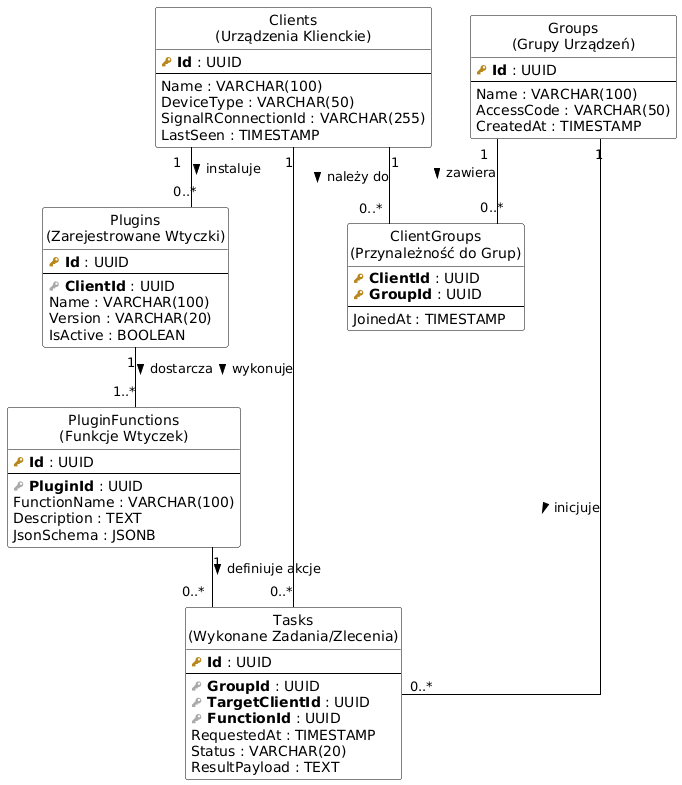
\includegraphics[width=0.8\textwidth]{figures/erd-diagram.png}
	\vspace{5cm}
	\caption{Diagram relacyjny bazy danych (ERD) systemu}
	\label{fig:erd_diagram}
\end{figure}
